\PassOptionsToPackage{unicode=true}{hyperref} % options for packages loaded elsewhere
\PassOptionsToPackage{hyphens}{url}
%
\documentclass[]{article}
\usepackage[a4paper,top=3cm,bottom=3cm,left=3cm,right=3cm,marginparwidth=1.75cm]{geometry}
\usepackage[UTF8]{ctex}
\usepackage{lmodern}
\usepackage{amssymb,amsmath}
\usepackage{ifxetex,ifluatex}
\usepackage{fixltx2e} % provides \textsubscript
\ifnum 0\ifxetex 1\fi\ifluatex 1\fi=0 % if pdftex
  \usepackage[T1]{fontenc}
  \usepackage[utf8]{inputenc}
  \usepackage{textcomp} % provides euro and other symbols
\else % if luatex or xelatex
  \usepackage{unicode-math}
  \defaultfontfeatures{Ligatures=TeX,Scale=MatchLowercase}
\fi
% use upquote if available, for straight quotes in verbatim environments
\IfFileExists{upquote.sty}{\usepackage{upquote}}{}
% use microtype if available
\IfFileExists{microtype.sty}{%
\usepackage[]{microtype}
\UseMicrotypeSet[protrusion]{basicmath} % disable protrusion for tt fonts
}{}
\IfFileExists{parskip.sty}{%
\usepackage{parskip}
}{% else
\setlength{\parindent}{0pt}
\setlength{\parskip}{6pt plus 2pt minus 1pt}
}
\usepackage{hyperref}
\hypersetup{
            pdfborder={0 0 0},
            breaklinks=true}
\urlstyle{same}  % don't use monospace font for urls
\usepackage{color}
\usepackage{fancyvrb}
\newcommand{\VerbBar}{|}
\newcommand{\VERB}{\Verb[commandchars=\\\{\}]}
\DefineVerbatimEnvironment{Highlighting}{Verbatim}{commandchars=\\\{\}}
% Add ',fontsize=\small' for more characters per line
\newenvironment{Shaded}{}{}
\newcommand{\AlertTok}[1]{\textcolor[rgb]{1.00,0.00,0.00}{\textbf{#1}}}
\newcommand{\AnnotationTok}[1]{\textcolor[rgb]{0.38,0.63,0.69}{\textbf{\textit{#1}}}}
\newcommand{\AttributeTok}[1]{\textcolor[rgb]{0.49,0.56,0.16}{#1}}
\newcommand{\BaseNTok}[1]{\textcolor[rgb]{0.25,0.63,0.44}{#1}}
\newcommand{\BuiltInTok}[1]{#1}
\newcommand{\CharTok}[1]{\textcolor[rgb]{0.25,0.44,0.63}{#1}}
\newcommand{\CommentTok}[1]{\textcolor[rgb]{0.38,0.63,0.69}{\textit{#1}}}
\newcommand{\CommentVarTok}[1]{\textcolor[rgb]{0.38,0.63,0.69}{\textbf{\textit{#1}}}}
\newcommand{\ConstantTok}[1]{\textcolor[rgb]{0.53,0.00,0.00}{#1}}
\newcommand{\ControlFlowTok}[1]{\textcolor[rgb]{0.00,0.44,0.13}{\textbf{#1}}}
\newcommand{\DataTypeTok}[1]{\textcolor[rgb]{0.56,0.13,0.00}{#1}}
\newcommand{\DecValTok}[1]{\textcolor[rgb]{0.25,0.63,0.44}{#1}}
\newcommand{\DocumentationTok}[1]{\textcolor[rgb]{0.73,0.13,0.13}{\textit{#1}}}
\newcommand{\ErrorTok}[1]{\textcolor[rgb]{1.00,0.00,0.00}{\textbf{#1}}}
\newcommand{\ExtensionTok}[1]{#1}
\newcommand{\FloatTok}[1]{\textcolor[rgb]{0.25,0.63,0.44}{#1}}
\newcommand{\FunctionTok}[1]{\textcolor[rgb]{0.02,0.16,0.49}{#1}}
\newcommand{\ImportTok}[1]{#1}
\newcommand{\InformationTok}[1]{\textcolor[rgb]{0.38,0.63,0.69}{\textbf{\textit{#1}}}}
\newcommand{\KeywordTok}[1]{\textcolor[rgb]{0.00,0.44,0.13}{\textbf{#1}}}
\newcommand{\NormalTok}[1]{#1}
\newcommand{\OperatorTok}[1]{\textcolor[rgb]{0.40,0.40,0.40}{#1}}
\newcommand{\OtherTok}[1]{\textcolor[rgb]{0.00,0.44,0.13}{#1}}
\newcommand{\PreprocessorTok}[1]{\textcolor[rgb]{0.74,0.48,0.00}{#1}}
\newcommand{\RegionMarkerTok}[1]{#1}
\newcommand{\SpecialCharTok}[1]{\textcolor[rgb]{0.25,0.44,0.63}{#1}}
\newcommand{\SpecialStringTok}[1]{\textcolor[rgb]{0.73,0.40,0.53}{#1}}
\newcommand{\StringTok}[1]{\textcolor[rgb]{0.25,0.44,0.63}{#1}}
\newcommand{\VariableTok}[1]{\textcolor[rgb]{0.10,0.09,0.49}{#1}}
\newcommand{\VerbatimStringTok}[1]{\textcolor[rgb]{0.25,0.44,0.63}{#1}}
\newcommand{\WarningTok}[1]{\textcolor[rgb]{0.38,0.63,0.69}{\textbf{\textit{#1}}}}
\usepackage{graphicx,grffile}
\makeatletter
\def\maxwidth{\ifdim\Gin@nat@width>\linewidth\linewidth\else\Gin@nat@width\fi}
\def\maxheight{\ifdim\Gin@nat@height>\textheight\textheight\else\Gin@nat@height\fi}
\makeatother
% Scale images if necessary, so that they will not overflow the page
% margins by default, and it is still possible to overwrite the defaults
% using explicit options in \includegraphics[width, height, ...]{}
\setkeys{Gin}{width=\maxwidth,height=\maxheight,keepaspectratio}
\setlength{\emergencystretch}{3em}  % prevent overfull lines
\providecommand{\tightlist}{%
  \setlength{\itemsep}{0pt}\setlength{\parskip}{0pt}}
\setcounter{secnumdepth}{0}
% Redefines (sub)paragraphs to behave more like sections
\ifx\paragraph\undefined\else
\let\oldparagraph\paragraph
\renewcommand{\paragraph}[1]{\oldparagraph{#1}\mbox{}}
\fi
\ifx\subparagraph\undefined\else
\let\oldsubparagraph\subparagraph
\renewcommand{\subparagraph}[1]{\oldsubparagraph{#1}\mbox{}}
\fi

% set default figure placement to htbp
\makeatletter
\def\fps@figure{htbp}
\makeatother


\title{数据结构与算法I 实验10}
\author{2019201409 于倬浩}
\begin{document}

\maketitle

\hypertarget{header-n25}{%
\subsection{1.Number of Islands}\label{header-n25}}

给出一个01矩阵,求1构成的连通块个数。

考虑到今天上课讲了并查集,尽管这道题可以使用BFS/DFS等多种更简单且运行效率更高的做法,现在强行使用并查集来做。

将每个位置视为一个元素,初始没有元素相交。接下来扫描每个格子,如果和当前格子相邻的格子都是,就将两个格子代表的元素合并。这样,扫描完成一遍后,所有连通块内每个元素都在同一集合内。

统计答案也比较简单,首先初始状态下,每个位置对答案的贡献都是1,即``有多少个1初始就有多少个连通块''。接下来每次合并时,将答案减一,表示两个集合合并,当前的集合数量减少1,这样合并完成后我们就得到了集合的数量。

即使使用路径压缩+按秩合并,程序的运行时间依旧是\(O(nm \times \alpha(nm))\),高于使用BFS/DFS的\(O(nm)\)时间复杂度,因此这道题使用并查集理论上运行效率更低,实际上常数因子也很大。

\begin{Shaded}
\begin{Highlighting}[]
\KeywordTok{class}\NormalTok{ Solution \{}
\KeywordTok{public}\NormalTok{:}
\NormalTok{    vector<}\DataTypeTok{int}\NormalTok{> fa; }\CommentTok{// 并查集数组}
    \DataTypeTok{int}\NormalTok{ n, m;}
    \PreprocessorTok{#define id(i, j) ((i) * m + (j))}
    \DataTypeTok{int}\NormalTok{ find(}\DataTypeTok{int}\NormalTok{ x) \{ }\CommentTok{// 路径压缩}
        \ControlFlowTok{return}\NormalTok{ fa[x] == x? fa[x] : (fa[x] = find(fa[x]));}
\NormalTok{    \}}
    \DataTypeTok{int}\NormalTok{ numIslands(vector<vector<}\DataTypeTok{char}\NormalTok{>>& grid) \{}
        \DataTypeTok{int}\NormalTok{ num = grid.size() * grid[}\DecValTok{0}\NormalTok{].size();}
\NormalTok{        n = grid.size(), m = grid[}\DecValTok{0}\NormalTok{].size();}
\NormalTok{        fa.clear();}
        \ControlFlowTok{for}\NormalTok{(}\DataTypeTok{int}\NormalTok{ i = }\DecValTok{0}\NormalTok{; i < num; ++i) fa.push_back(i);}
        \DataTypeTok{int}\NormalTok{ land = }\DecValTok{0}\NormalTok{;}
        \ControlFlowTok{for}\NormalTok{(}\DataTypeTok{int}\NormalTok{ i = }\DecValTok{0}\NormalTok{; i < n; ++i) \{}
            \ControlFlowTok{for}\NormalTok{(}\DataTypeTok{int}\NormalTok{ j = }\DecValTok{0}\NormalTok{; j < m; ++j) }\ControlFlowTok{if}\NormalTok{(grid[i][j] == }\CharTok{'1'}\NormalTok{) \{ }\CommentTok{//扫描每个1}
\NormalTok{                ++land; }\CommentTok{//初始每个位置都有1的贡献}
                \ControlFlowTok{if}\NormalTok{(i + }\DecValTok{1}\NormalTok{ < n && grid[i + }\DecValTok{1}\NormalTok{][j] == }\CharTok{'1'}\NormalTok{) \{}
                    \DataTypeTok{int}\NormalTok{ f1 = find(id(i, j)), f2 = find(id(i + }\DecValTok{1}\NormalTok{, j));}
                    \ControlFlowTok{if}\NormalTok{(f1 != f2)\{ }\CommentTok{//合并两个连通块,连通块数量-1}
\NormalTok{                        --land;}
\NormalTok{                        fa[f2] = f1;}
\NormalTok{                    \}}
\NormalTok{                \}}
                \ControlFlowTok{if}\NormalTok{(j + }\DecValTok{1}\NormalTok{ < m && grid[i][j + }\DecValTok{1}\NormalTok{] == }\CharTok{'1'}\NormalTok{) \{}
                    \DataTypeTok{int}\NormalTok{ f1 = find(id(i, j)), f2 = find(id(i, j + }\DecValTok{1}\NormalTok{));}
                    \ControlFlowTok{if}\NormalTok{(f1 != f2)\{}
\NormalTok{                        --land;}
\NormalTok{                        fa[f2] = f1;}
\NormalTok{                    \}}
\NormalTok{                \}}
\NormalTok{            \}}
\NormalTok{        \}}
        \ControlFlowTok{return}\NormalTok{ land;}
\NormalTok{    \}}
\NormalTok{\};}
\end{Highlighting}
\end{Shaded}


\begin{figure}
    \centering
    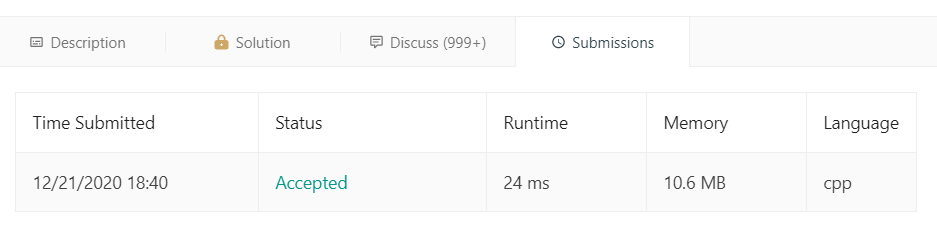
\includegraphics{C:/Users/zhuoh/Desktop/Docs/ds-lab10/ds-10.assets/image-20201223155127170.png}
    \caption{Number of Islands}
\end{figure}

\hypertarget{header-n34}{%
\subsection{2. Longest Consecutive Sequence}\label{header-n34}}

首先强行考虑使用并查集的思路。对值域维护并查集,初始将每个元素视为一个单元素集合,接下来尝试合并值域上相邻的元素即可。然而,题目中给出值域范围又很大(1e9),不可能对值域开一个数组,因此必须使用哈希表来代替数组。

到现在,算法的时间复杂度为\(O(n\alpha(n) \times (1 + \alpha))\),其中第二个\(\alpha\)表示哈希表的装载因子,已经不是非常优秀了。

实际上,如果必须使用哈希表这一数据结构,再使用并查集就显得有些多此一举了。

我们只需要使用哈希表存储所有的\(n\)个元素。接下来,遍历哈希表中的每个元素。假设当前遍历到的元素为\(x\),如果\(x-1\)在哈希表中不存在,就开始查找过程:每次判断\(x+k\)是否存在于哈希表中,如果存在就\(k = k + 1\),否则当前一段的连续的值域区间长度即为\(k\)。如果\(x-1\)在哈希表中存在,那么直接跳过这个元素,因为每一个值域连续的段,我们只需要考虑一次。

这样,算法的时间复杂度即为\(O(n\times(1 + \alpha))\),省去了并查集多余的一步,代码也简单得多。(实际上这些做法的常数因子都太大了,对于题目数据\(n\)只有\(10^4\)来说,\texttt{std::sort}跑的最快)。

\begin{Shaded}
\begin{Highlighting}[]
\KeywordTok{class}\NormalTok{ Solution \{}
\KeywordTok{public}\NormalTok{:}
\NormalTok{    unordered_set<}\DataTypeTok{int}\NormalTok{> st; }\CommentTok{//使用stl自带的哈希表}
    \DataTypeTok{int}\NormalTok{ longestConsecutive(vector<}\DataTypeTok{int}\NormalTok{>& nums) \{}
        \ControlFlowTok{for}\NormalTok{(}\KeywordTok{auto}\NormalTok{ i:nums) st.insert(i); }\CommentTok{//将所有元素插入哈希表}
        \DataTypeTok{int}\NormalTok{ ans = }\DecValTok{0}\NormalTok{;}
        \ControlFlowTok{for}\NormalTok{(}\KeywordTok{auto}\NormalTok{ i:st) }\ControlFlowTok{if}\NormalTok{(!st.count(i - }\DecValTok{1}\NormalTok{)) \{}
            \CommentTok{//枚举每个连续段的开头}
            \DataTypeTok{int}\NormalTok{ cur = i, num = }\DecValTok{1}\NormalTok{;}
            \ControlFlowTok{while}\NormalTok{(st.count(cur + }\DecValTok{1}\NormalTok{)) ++cur, ++num;}
            \ControlFlowTok{if}\NormalTok{(num > ans) ans = num;}
\NormalTok{        \}}
        \ControlFlowTok{return}\NormalTok{ ans;}
\NormalTok{    \}}
\NormalTok{\};}
\end{Highlighting}
\end{Shaded}

\begin{figure}
\centering
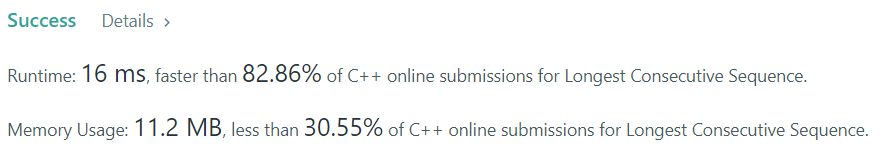
\includegraphics{C:/Users/zhuoh/Desktop/Docs/ds-lab10/ds-10.assets/image-20201223165219499.png}
\caption{使用哈希表的提交记录}
\end{figure}

当然为了完成实验要求,还是强行写了使用哈希表+并查集的代码:

\begin{Shaded}
\begin{Highlighting}[]
\KeywordTok{class}\NormalTok{ Solution \{}
\KeywordTok{public}\NormalTok{:}
\NormalTok{    unordered_map<}\DataTypeTok{int}\NormalTok{, }\DataTypeTok{int}\NormalTok{> mp;}
\NormalTok{    vector<}\DataTypeTok{int}\NormalTok{> fa, rk, sz;}
    \DataTypeTok{int}\NormalTok{ n;}
    \DataTypeTok{int}\NormalTok{ find(}\DataTypeTok{int}\NormalTok{ x) \{}
        \ControlFlowTok{return}\NormalTok{ x == fa[x] ? x : fa[x] = find(fa[x]);}
\NormalTok{    \}}
    \KeywordTok{inline} \DataTypeTok{void}\NormalTok{ merge(}\DataTypeTok{int}\NormalTok{ a, }\DataTypeTok{int}\NormalTok{ b) \{ }\CommentTok{//按秩合并+路径压缩}
        \DataTypeTok{int}\NormalTok{ f1 = find(a), f2 = find(b);}
        \ControlFlowTok{if}\NormalTok{(f1 == f2) }\ControlFlowTok{return}\NormalTok{;}
        \ControlFlowTok{if}\NormalTok{(rk[f1] < rk[f2]) swap(f1, f2);}
\NormalTok{        fa[f2] = f1, sz[f1] += sz[f2];}
        \ControlFlowTok{if}\NormalTok{(rk[f1] == rk[f2]) ++rk[f1];}
\NormalTok{    \}}
    \DataTypeTok{int}\NormalTok{ longestConsecutive(vector<}\DataTypeTok{int}\NormalTok{>& nums) \{}
\NormalTok{        n = nums.size();}
\NormalTok{        fa.resize(n), sz.resize(n), rk.resize(n);}
        \ControlFlowTok{for}\NormalTok{(}\DataTypeTok{int}\NormalTok{ i = }\DecValTok{0}\NormalTok{; i < n; ++i) \{}
            \ControlFlowTok{if}\NormalTok{(mp.count(nums[i])) }\ControlFlowTok{continue}\NormalTok{; }\CommentTok{//处理重复元素}
\NormalTok{            mp[nums[i]] = i;}
\NormalTok{            fa[i] = i, sz[i] = }\DecValTok{1}\NormalTok{, rk[i] = }\DecValTok{0}\NormalTok{;}
\NormalTok{        \}}
        \ControlFlowTok{for}\NormalTok{(}\DataTypeTok{int}\NormalTok{ i = }\DecValTok{0}\NormalTok{; i < n; ++i) \{}
            \ControlFlowTok{if}\NormalTok{(mp[nums[i]] != i) }\ControlFlowTok{continue}\NormalTok{; }\CommentTok{//处理重复元素}
            \ControlFlowTok{if}\NormalTok{(mp.count(nums[i] - }\DecValTok{1}\NormalTok{)) \{ }\CommentTok{//查看值域上相邻元素}
                \DataTypeTok{int}\NormalTok{ t = mp[nums[i] - }\DecValTok{1}\NormalTok{];}
\NormalTok{                merge(t, i);}
\NormalTok{            \}}
            \ControlFlowTok{if}\NormalTok{(mp.count(nums[i] + }\DecValTok{1}\NormalTok{)) \{ }\CommentTok{//查看值域上相邻元素}
                \DataTypeTok{int}\NormalTok{ t = mp[nums[i] + }\DecValTok{1}\NormalTok{];}
\NormalTok{                merge(t, i);}
\NormalTok{            \}}
\NormalTok{        \}}
        \DataTypeTok{int}\NormalTok{ ans = }\DecValTok{0}\NormalTok{; }\CommentTok{//统计答案}
        \ControlFlowTok{for}\NormalTok{(}\DataTypeTok{int}\NormalTok{ i = }\DecValTok{0}\NormalTok{; i < n; ++i) ans = ans < sz[i] ? sz[i] : ans;}
        
        \ControlFlowTok{return}\NormalTok{ ans;}
\NormalTok{    \}}
\NormalTok{\};}
\end{Highlighting}
\end{Shaded}

\begin{figure}
\centering
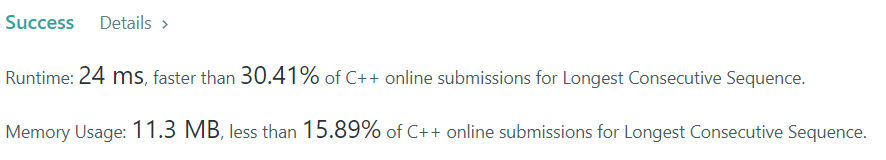
\includegraphics{C:/Users/zhuoh/Desktop/Docs/ds-lab10/ds-10.assets/image-20201223165131661.png}
\caption{使用哈希表+并查集的提交记录}
\end{figure}

\end{document}
